% Chapter 0: Fundamentals of Time Series Analysis
% Harvard-quality academic presentation
% Bachelor's program, Bucharest University of Economic Studies

\documentclass[9pt, aspectratio=169, t]{beamer}

% Ensure content fits on slides
\setbeamersize{text margin left=8mm, text margin right=8mm}

%=============================================================================
% THEME AND STYLE CONFIGURATION
%=============================================================================
\usetheme{default}
% Using default theme for clean header/footer control

% Color Palette (matching Redispatch PDF)
\definecolor{MainBlue}{RGB}{26, 58, 110}
\definecolor{AccentBlue}{RGB}{26, 58, 110}
\definecolor{IDAred}{RGB}{205, 0, 0}
\definecolor{DarkGray}{RGB}{51, 51, 51}
\definecolor{MediumGray}{RGB}{128, 128, 128}
\definecolor{LightGray}{RGB}{248, 248, 248}
\definecolor{VeryLightGray}{RGB}{235, 235, 235}
\definecolor{KeynoteGray}{RGB}{218, 218, 218}
\definecolor{SectionGray}{RGB}{120, 120, 120}
\definecolor{FooterGray}{RGB}{100, 100, 100}
\definecolor{Crimson}{RGB}{220, 53, 69}
\definecolor{Forest}{RGB}{46, 125, 50}
\definecolor{Amber}{RGB}{181, 133, 63}
\definecolor{Orange}{RGB}{230, 126, 34}
\definecolor{Purple}{RGB}{142, 68, 173}

% Gradient background (exact Keynote 315° gradient: white to RGB 218,218,218)
\setbeamertemplate{background}{%
    \begin{tikzpicture}[remember picture, overlay]
        \shade[shading=axis, shading angle=315,
        top color=white, bottom color=KeynoteGray]
        (current page.south west) rectangle (current page.north east);
    \end{tikzpicture}%
}
% Fallback solid color for compatibility
\setbeamercolor{background canvas}{bg=}

\setbeamercolor{palette primary}{bg=MainBlue, fg=white}
\setbeamercolor{palette secondary}{bg=MainBlue!85, fg=white}
\setbeamercolor{palette tertiary}{bg=MainBlue!70, fg=white}
\setbeamercolor{structure}{fg=MainBlue}
\setbeamercolor{title}{fg=IDAred}
\setbeamercolor{frametitle}{fg=IDAred, bg=}
\setbeamercolor{block title}{bg=MainBlue, fg=white}
\setbeamercolor{block body}{bg=VeryLightGray, fg=DarkGray}
\setbeamercolor{block title alerted}{bg=Crimson, fg=white}
\setbeamercolor{block body alerted}{bg=Crimson!8, fg=DarkGray}
\setbeamercolor{block title example}{bg=Forest, fg=white}
\setbeamercolor{block body example}{bg=Forest!8, fg=DarkGray}
\setbeamercolor{item}{fg=MainBlue}

% Footer colors (override Madrid theme blue)
\setbeamercolor{author in head/foot}{fg=FooterGray, bg=}
\setbeamercolor{title in head/foot}{fg=FooterGray, bg=}
\setbeamercolor{date in head/foot}{fg=FooterGray, bg=}
\setbeamercolor{section in head/foot}{fg=FooterGray, bg=}
\setbeamercolor{subsection in head/foot}{fg=FooterGray, bg=}

% Bullet styles (apply everywhere including blocks)
\setbeamertemplate{itemize item}{\color{MainBlue}$\boxdot$}
\setbeamertemplate{itemize subitem}{\color{MainBlue}$\blacktriangleright$}
\setbeamertemplate{itemize subsubitem}{\color{MainBlue}\tiny$\bullet$}
\setbeamertemplate{itemize/enumerate body begin}{\normalsize}
\setbeamertemplate{itemize/enumerate subbody begin}{\normalsize}

% Item spacing - compact style
\setlength{\leftmargini}{10pt}       % Level 1: minimal indent
\setlength{\leftmarginii}{10pt}      % Level 2: minimal additional indent
% Compact list spacing (zero extra space before/after lists in blocks)
\makeatletter
\def\@listi{\leftmargin\leftmargini \topsep 0pt \parsep 0pt \itemsep 0pt}
\def\@listii{\leftmargin\leftmarginii \topsep 0pt \parsep 0pt \itemsep 0pt}
\makeatother

\setbeamertemplate{navigation symbols}{}

%=============================================================================
% CUSTOM HEADLINE
%=============================================================================
\setbeamertemplate{headline}{%
    \vskip10pt%
    \hbox to \paperwidth{%
        \hskip0.5cm%
        {\small\color{FooterGray}\renewcommand{\hyperlink}[2]{##2}\insertsectionhead}%
        \hfill%
        \textcolor{FooterGray}{\small\insertframenumber}%
        \hskip0.5cm%
    }%
    \vskip4pt%
    {\color{FooterGray}\hrule height 0.4pt}%
}

%=============================================================================
% CUSTOM FOOTER
%=============================================================================
\usepackage{fontawesome5}

\setbeamertemplate{footline}{%
    {\color{FooterGray}\hrule height 0.4pt}%
    \vskip4pt%
    \hbox to \paperwidth{%
        \hskip0.5cm%
        \textcolor{FooterGray}{\small Time Series Analysis and Forecasting}%
        \hfill%
        \raisebox{-0.1em}{%
            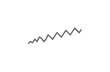
\begin{tikzpicture}[x=0.08em, y=0.08em, line width=0.4pt]
                \draw[FooterGray] (0,3) -- (1,4) -- (2,3.5) -- (3,5) -- (4,4) -- (5,6) -- (6,5.5) -- (7,4) -- (8,5) -- (9,7) -- (10,6) -- (11,5) -- (12,6.5) -- (13,8) -- (14,7) -- (15,6) -- (16,7.5) -- (17,9) -- (18,8) -- (19,7) -- (20,8.5) -- (21,10) -- (22,9) -- (23,8) -- (24,9.5);
            \end{tikzpicture}%
        }%
        \hskip0.5cm%
    }%
    \vskip6pt%
}

%=============================================================================
% PACKAGES
%=============================================================================
\usepackage[utf8]{inputenc}
\usepackage[T1]{fontenc}
\usepackage{amsmath, amssymb, amsthm}
\usepackage{mathtools}
\usepackage{bm}
\usepackage{tikz}
\usetikzlibrary{arrows.meta, positioning, shapes, calc, decorations.pathreplacing, shadings}
\usepackage{booktabs}
\usepackage{multirow}
\usepackage{array}
\usepackage{graphicx}
\usepackage{hyperref}
\usepackage{colortbl}
\hypersetup{colorlinks=true, linkcolor=MainBlue, urlcolor=MainBlue}
\graphicspath{{../../logos/}{../../charts/}}
\hfuzz=2pt  % Suppress tiny overfull warnings (<2pt)
\vfuzz=2pt  % Suppress tiny vertical overfull warnings (<2pt)

%=============================================================================
% QUANTLET COMMAND
%=============================================================================
\newcommand{\quantlet}[2]{%
    \hfill\href{#2}{%
        \raisebox{-0.15em}{\includegraphics[height=0.7em]{ql_logo.png}}%
        \textcolor{MainBlue}{\tiny\ #1}%
    }%
}

%=============================================================================
% CUSTOM TITLE PAGE
%=============================================================================
\defbeamertemplate*{title page}{hybrid}[1][]
{
    \vspace{0.2cm}
    % Logos row - top header (with clickable links)
    \begin{center}
        \href{https://www.ase.ro}{\includegraphics[height=1.0cm]{ase_logo.png}}\hspace{0.3cm}%
        \href{https://theida.net}{\includegraphics[height=1.0cm]{ida_logo.png}}\hspace{0.3cm}%
        \href{https://blockchain-research-center.com}{\includegraphics[height=1.0cm]{brc_logo.png}}\hspace{0.3cm}%
        \href{https://www.ai4efin.ase.ro}{\includegraphics[height=1.0cm]{ai4efin_logo.png}}\hspace{0.3cm}%
        \href{https://ipe.ro/new}{\includegraphics[height=1.0cm]{acad_logo.png}}\hspace{0.3cm}%
        \href{https://www.digital-finance-msca.com}{\includegraphics[height=1.0cm]{msca_logo.png}}%
    \end{center}

    \vspace{0.6cm}

    % Main title with Q logos on sides (with clickable links)
    \begin{center}
        \begin{minipage}{0.1\textwidth}
            \centering
            \href{https://quantlet.com}{\includegraphics[height=1.1cm]{ql_logo.png}}
        \end{minipage}%
        \begin{minipage}{0.78\textwidth}
            \centering
            {\LARGE\bfseries\usebeamercolor[fg]{title}\inserttitle}

            \vspace{0.3cm}

            {\usebeamerfont{subtitle}\usebeamercolor[fg]{title}\insertsubtitle}
        \end{minipage}%
        \begin{minipage}{0.1\textwidth}
            \centering
            \href{https://quantinar.com}{\includegraphics[height=1.1cm]{qr_logo.png}}
        \end{minipage}
    \end{center}

    \vspace{0.6cm}

    % Authors (left aligned)
    \hspace{0.5cm}{\usebeamerfont{author}\insertauthor}

    \vspace{0.3cm}

    % Institute/Affiliations (left aligned)
    \hspace{0.5cm}\begin{minipage}[t]{0.9\textwidth}
        \raggedright\small\insertinstitute
    \end{minipage}
}

%=============================================================================
% THEOREM ENVIRONMENTS
%=============================================================================
\theoremstyle{definition}
\setbeamertemplate{theorems}[numbered]
\newtheorem{defn}{Definition}
\newtheorem{thm}{Theorem}
\newtheorem{prop}{Proposition}
\newtheorem{rmk}{Remark}

%=============================================================================
% CUSTOM COMMANDS
%=============================================================================
\newcommand{\E}{\mathbb{E}}
\newcommand{\Var}{\text{Var}}
\newcommand{\Cov}{\text{Cov}}
\newcommand{\Corr}{\text{Corr}}
\newcommand{\R}{\mathbb{R}}
\newcommand{\N}{\mathbb{N}}
\newcommand{\Z}{\mathbb{Z}}
\newcommand{\B}{\mathbf{B}}
\newcommand{\imark}{\textcolor{MainBlue}{\textbullet}}
\newcommand{\RMSE}{\text{RMSE}}
\newcommand{\MAE}{\text{MAE}}
\newcommand{\MAPE}{\text{MAPE}}

%=============================================================================
% TITLE INFORMATION
%=============================================================================
\title[Time Series Analysis]{Time Series Analysis and Forecasting}
\subtitle{Chapter 0: Fundamentals}
\author[D.T. Pele]{Daniel Traian PELE}
\institute{Bucharest University of Economic Studies\\
IDA Institute Digital Assets\\
Blockchain Research Center\\
AI4EFin Artificial Intelligence for Energy Finance\\
Romanian Academy, Institute for Economic Forecasting\\
MSCA Digital Finance}
\date{}

\begin{document}

% Title page (no header/footer)
{
\setbeamertemplate{headline}{}
\setbeamertemplate{footline}{}
\begin{frame}
    \titlepage
\end{frame}
}

%=============================================================================
% LEARNING OBJECTIVES
%=============================================================================
\begin{frame}{Learning Objectives}
    \begin{block}{By the end of this chapter, you will be able to:}
        \begin{itemize}\setlength{\itemsep}{2pt}
            \item[\textcolor{MainBlue}{\textbf{1.}}] \textbf{Define} time series and distinguish them from cross-sectional and panel data
            \item[\textcolor{MainBlue}{\textbf{2.}}] \textbf{Decompose} time series into trend-cycle, seasonality, and residual components
            \item[\textcolor{MainBlue}{\textbf{3.}}] \textbf{Apply} exponential smoothing methods (SES, Holt, Holt-Winters, ETS)
            \item[\textcolor{MainBlue}{\textbf{4.}}] \textbf{Evaluate} forecasts using MAE, RMSE, MAPE, sMAPE
            \item[\textcolor{MainBlue}{\textbf{5.}}] \textbf{Implement} train/validation/test splitting and cross-validation
            \item[\textcolor{MainBlue}{\textbf{6.}}] \textbf{Model} seasonality using dummy variables or Fourier terms
            \item[\textcolor{MainBlue}{\textbf{7.}}] \textbf{Remove} trend and seasonality through appropriate methods
            \item[\textcolor{MainBlue}{\textbf{8.}}] \textbf{Distinguish} between deterministic and stochastic trends
        \end{itemize}
    \end{block}
\end{frame}

%=============================================================================
% DATA SOURCES AND SOFTWARE TOOLS
%=============================================================================
\begin{frame}{Data Sources and Software Tools}
    \begin{columns}[T]
        \begin{column}{0.48\textwidth}
            \begin{block}{Data Sources}
                \begin{itemize}\setlength{\itemsep}{0pt}
                    \item \textbf{Yahoo Finance}
                    \begin{itemize}
                        \item Stock prices, cryptocurrencies, exchange rates
                    \end{itemize}
                    \item \textbf{FRED} (Federal Reserve)
                    \begin{itemize}
                        \item GDP, unemployment, interest rates
                    \end{itemize}
                    \item \textbf{Eurostat / INS / BNR}
                    \begin{itemize}
                        \item European and Romanian economic data
                    \end{itemize}
                    \item \textbf{Classic datasets}
                    \begin{itemize}
                        \item AirPassengers, Sunspots, CO$_2$
                    \end{itemize}
                \end{itemize}
            \end{block}
        \end{column}
        \begin{column}{0.48\textwidth}
            \begin{exampleblock}{Python}
                \begin{itemize}\setlength{\itemsep}{0pt}
                    \item \texttt{yfinance} — Yahoo Finance data
                    \item \texttt{pandas\_datareader} — FRED, Eurostat
                    \item \texttt{statsmodels} — statistical models
                    \item \texttt{pandas} — data manipulation
                    \item \texttt{matplotlib} — visualization
                \end{itemize}
            \end{exampleblock}
            \vspace{0.1cm}
            \begin{alertblock}{R}
                \begin{itemize}\setlength{\itemsep}{0pt}
                    \item \texttt{quantmod} — financial data
                    \item \texttt{tseries} — time series tests
                    \item \texttt{forecast} — forecasting models
                    \item \texttt{fredr} — FRED API access
                \end{itemize}
            \end{alertblock}
        \end{column}
    \end{columns}
\end{frame}

%=============================================================================
% TABLE OF CONTENTS
%=============================================================================
\begin{frame}{Chapter Outline}
    \setbeamertemplate{section in toc}{\color{MainBlue}$\boxdot$~\inserttocsection}
    \tableofcontents
\end{frame}

%=============================================================================
% MOTIVATION
%=============================================================================
\section{Motivation}

\begin{frame}{Time Series Are Everywhere}
    \vspace{-0.3cm}
    \begin{center}
        \includegraphics[width=0.95\textwidth, height=0.60\textheight, keepaspectratio]{ch1_motivation_everywhere.png}
    \end{center}
    \vspace{-2mm}
    \quantlet{TSA\_ch0\_real\_data}{https://github.com/QuantLet/TSA/tree/main/TSA_ch0/TSA_ch0_real_data}
    \vspace{-0.2cm}
    {\footnotesize
    \begin{itemize}
        \item \textbf{Finance}: Stock prices, exchange rates, volumes
        \item \textbf{Economics}: GDP, unemployment, inflation rates
        \item \textbf{Business}: Sales, website traffic, demand
        \item \textbf{Science}: Temperature, pollution, vital signs
    \end{itemize}
    }
\end{frame}

\begin{frame}{Why Do We Study Time Series?}
    \vspace{-0.2cm}
    \begin{center}
        \includegraphics[width=0.95\textwidth, height=0.52\textheight, keepaspectratio]{ch1_motivation_forecast.png}
    \end{center}
    \vspace{-2mm}
    \quantlet{TSA\_ch0\_real\_data}{https://github.com/QuantLet/TSA/tree/main/TSA_ch0/TSA_ch0_real_data}
    \vspace{-0.3cm}
    {\footnotesize
    \begin{alertblock}{Main objective: forecasting}
        \begin{itemize}\setlength{\itemsep}{0pt}
            \item We use historical patterns to predict future values $\rightarrow$ essential for business planning, risk management, and policy decisions
        \end{itemize}
    \end{alertblock}
    }
\end{frame}

\begin{frame}{Understanding Time Series Structure}
    \vspace{-0.2cm}
    \begin{center}
        \includegraphics[width=0.92\textwidth, height=0.52\textheight, keepaspectratio]{ch1_motivation_components.png}
    \end{center}
    \vspace{-2mm}
    \quantlet{TSA\_ch0\_real\_data}{https://github.com/QuantLet/TSA/tree/main/TSA_ch0/TSA_ch0_real_data}
    \vspace{-0.3cm}
    {\footnotesize
    \begin{exampleblock}{Decomposition}
        \begin{itemize}\setlength{\itemsep}{0pt}
            \item Any time series can be decomposed into: \textbf{trend-cycle} + \textbf{seasonality} + \textbf{noise}
        \end{itemize}
    \end{exampleblock}
    }
\end{frame}

%=============================================================================
% SECTION 1: WHAT IS A TIME SERIES
%=============================================================================
\section{What Is a Time Series?}

\begin{frame}{Definition of a Time Series}
    \begin{defn}[Time Series]
        \begin{itemize}\setlength{\itemsep}{0pt}
            \item \textbf{Time series}: a sequence of observations $\{X_t\}$ indexed by time:
            $\{X_t : t \in \mathcal{T}\}$
            where $\mathcal{T}$ is a set of indices representing time points
        \end{itemize}
    \end{defn}

    \vspace{0.2cm}

    \begin{columns}[T]
        \column{0.5\textwidth}
        \begin{block}{Key Characteristics}
            \begin{itemize}\setlength{\itemsep}{0pt}
                \item \textbf{Ordered}: natural temporal order
                \item \textbf{Dependent}: consecutive observations are correlated
                \item \textbf{Discrete/Continuous}: $t = 1, 2, 3, \ldots$
            \end{itemize}
        \end{block}

        \column{0.5\textwidth}
        \begin{exampleblock}{Notation}
            \begin{itemize}\setlength{\itemsep}{0pt}
                \item \textbf{$X_t$}: observation at time $t$
                \item \textbf{$\{X_t\}_{t=1}^{T}$}: series with $T$ observations
            \end{itemize}
        \end{exampleblock}
    \end{columns}
\end{frame}

\begin{frame}{Time Series: Conceptual Illustration}
    \vspace{0.3cm}
    \begin{center}
        \includegraphics[width=0.75\textwidth, height=0.38\textheight, keepaspectratio]{ch1_def_timeseries.pdf}
    \end{center}
    \vspace{-0.1cm}
    \quantlet{TSA\_ch0\_definition}{https://github.com/QuantLet/TSA/tree/main/TSA_ch0/TSA_ch0_definition}
    \begin{exampleblock}{Fundamental Elements}
        \begin{itemize}\setlength{\itemsep}{0pt}
            \item \textbf{Formal notation}: $X_t$ = value at time $t$, $t \in \{1, 2, \ldots, T\}$
            \item \textbf{Autocorrelation}: $\rho_k = \text{Corr}(X_t, X_{t-k})$ --- measures temporal dependence
        \end{itemize}
    \end{exampleblock}
\end{frame}

\begin{frame}{Common Patterns in Time Series}
    \vspace{0.3cm}
    \begin{center}
        \includegraphics[width=0.75\textwidth, height=0.38\textheight, keepaspectratio]{ch1_ts_patterns.pdf}
    \end{center}
    \vspace{-0.1cm}
    \quantlet{TSA\_ch0\_definition}{https://github.com/QuantLet/TSA/tree/main/TSA_ch0/TSA_ch0_definition}
    \begin{block}{Types of Patterns}
        \begin{itemize}\setlength{\itemsep}{0pt}
            \item \textbf{Trend}: long-term increase or decrease
            \item \textbf{Seasonal}: regular periodic patterns
            \item \textbf{Cyclical}: medium-term fluctuations (2--10 years)
            \item \textbf{Random}: unpredictable fluctuations
        \end{itemize}
    \end{block}
\end{frame}

\begin{frame}{Practical Example: Real Financial Data}
    \vspace{0.3cm}
    \begin{center}
        \includegraphics[width=0.75\textwidth, height=0.38\textheight, keepaspectratio]{timeseries_definition.pdf}
    \end{center}
    \vspace{-0.1cm}
    \quantlet{TSA\_ch0\_definition}{https://github.com/QuantLet/TSA/tree/main/TSA_ch0/TSA_ch0_definition}
    \begin{block}{S\&P 500 (2024)}
        \begin{itemize}\setlength{\itemsep}{0pt}
            \item \textbf{Daily frequency}: $\approx$ 252 trading days/year
            \item \textbf{Observed characteristics}: upward trend, volatility clustering, persistence (momentum)
        \end{itemize}
    \end{block}
\end{frame}

\begin{frame}{Data Types: Comparison}
    \begin{center}
        \includegraphics[width=0.95\textwidth, height=0.52\textheight, keepaspectratio]{data_types_comparison.png}
    \end{center}
    \vspace{-0.2cm}
    \begin{center}
    \small
    \begin{tabular}{lccc}
        \toprule
        \textbf{Data Type} & \textbf{Units ($N$)} & \textbf{Time ($T$)} & \textbf{Example} \\
        \midrule
        Cross-sectional & Many & 1 & Survey of 1000 households \\
        Time series & 1 & Many & Daily S\&P 500 prices \\
        Panel & Many & Many & GDP of 50 countries, 20 years \\
        \bottomrule
    \end{tabular}
    \end{center}
    \vspace{-2mm}
    \quantlet{TSA\_ch0\_definition}{https://github.com/QuantLet/TSA/tree/main/TSA_ch0/TSA_ch0_definition}
\end{frame}

\begin{frame}{Examples of Time Series Data}
    \vspace{0.3cm}
    \begin{center}
        \includegraphics[width=0.75\textwidth, height=0.38\textheight, keepaspectratio]{multiple_assets.pdf}
    \end{center}
    \vspace{-0.1cm}
    \quantlet{TSA\_ch0\_real\_data}{https://github.com/QuantLet/TSA/tree/main/TSA_ch0/TSA_ch0_real_data}
    \begin{exampleblock}{Real financial data}
        \begin{itemize}\setlength{\itemsep}{0pt}
            \item \textbf{Source}: Yahoo Finance (2019--2025), normalized to base 100
            \item \textbf{Bitcoin}: most volatile; \textbf{Gold}: most stable
        \end{itemize}
    \end{exampleblock}
\end{frame}

%=============================================================================
% SECTION 2: TIME SERIES DECOMPOSITION
%=============================================================================
\section{Time Series Decomposition}

\begin{frame}{Why Do We Decompose a Time Series?}
    \vspace{-0.2cm}
    \begin{columns}[T]
        \begin{column}{0.48\textwidth}
            \begin{block}{Objectives}
                \begin{itemize}\setlength{\itemsep}{0pt}
                    \item Understanding underlying patterns
                    \item Removing seasonality for modeling
                    \item Identifying trend direction
                    \item Isolating irregular fluctuations
                    \item Improving forecast accuracy
                \end{itemize}
            \end{block}
        \end{column}
        \begin{column}{0.48\textwidth}
            \begin{exampleblock}{Components}
                \begin{itemize}\setlength{\itemsep}{0pt}
                    \item \textbf{$T_t$}: Trend-Cycle
                    \begin{itemize}
                        \item Long-term movement
                    \end{itemize}
                    \item \textbf{$S_t$}: Seasonal
                    \begin{itemize}
                        \item Regular periodic pattern
                    \end{itemize}
                    \item \textbf{$\varepsilon_t$}: Residual
                    \begin{itemize}
                        \item Random noise
                    \end{itemize}
                \end{itemize}
            \end{exampleblock}
        \end{column}
    \end{columns}

    \vspace{0.1cm}

    \begin{block}{Classical decomposition models}
        \begin{itemize}\setlength{\itemsep}{0pt}
            \item \textbf{Additive}: $X_t = T_t + S_t + \varepsilon_t$
            \begin{itemize}
                \item Constant seasonal amplitude
            \end{itemize}
            \item \textbf{Multiplicative}: $X_t = T_t \times S_t \times \varepsilon_t$
            \begin{itemize}
                \item Seasonal amplitude grows with the level
            \end{itemize}
        \end{itemize}
    \end{block}
\end{frame}

\begin{frame}{Time Series Decomposition: Visual Example}
    \vspace{0.3cm}
    \begin{center}
        \includegraphics[width=0.75\textwidth, height=0.38\textheight, keepaspectratio]{ch1_decomposition.png}
    \end{center}
    \vspace{-0.1cm}
    \quantlet{TSA\_ch0\_decomposition}{https://github.com/QuantLet/TSA/tree/main/TSA_ch0/TSA_ch0_decomposition}
    \begin{block}{Components Explained}
        \begin{itemize}\setlength{\itemsep}{0pt}
            \item \textbf{Original}: observed series
            \item \textbf{Trend-Cycle}: long-term movement
            \item \textbf{Seasonal}: periodic pattern
            \item \textbf{Residual}: random noise
        \end{itemize}
    \end{block}
\end{frame}

\begin{frame}{The Cyclical Component}
    \vspace{-0.3cm}
    \begin{center}
        \includegraphics[width=0.95\textwidth, height=0.50\textheight, keepaspectratio]{ch1_cyclical_component.png}
    \end{center}
        \vspace{-2mm}
        \quantlet{TSA\_ch0\_decomposition}{https://github.com/QuantLet/TSA/tree/main/TSA_ch0/TSA_ch0_decomposition}
    \vspace{-0.2cm}
    {\small
    \begin{columns}[T]
        \column{0.48\textwidth}
        \begin{block}{Characteristics}
            \begin{itemize}\setlength{\itemsep}{0pt}
                \item \textbf{Duration}: medium-term fluctuations (2--10 years)
                \item \textbf{Aperiodic}: no fixed period (vs seasonality)
                \item \textbf{Origin}: reflects business cycles
            \end{itemize}
        \end{block}

        \column{0.48\textwidth}
        \begin{alertblock}{In Practice}
            \begin{itemize}\setlength{\itemsep}{0pt}
                \item \textbf{Combination}: cycle combined with trend
                \item \textbf{Difficulty}: hard to identify in short series
                \item \textbf{Solution}: usually absorbed into trend-cycle
            \end{itemize}
        \end{alertblock}
    \end{columns}
    }
\end{frame}

\begin{frame}{The Additive Decomposition Model}
    \begin{block}{Model}
        \begin{itemize}\setlength{\itemsep}{0pt}
            \item \textbf{Equation}: $X_t = T_t + S_t + \varepsilon_t$
            \begin{itemize}
                \item Components are added together to form the observed series
            \end{itemize}
        \end{itemize}
    \end{block}

    \vspace{0.2cm}

    \begin{columns}[T]
        \column{0.48\textwidth}
        \begin{exampleblock}{When to Use}
            \begin{itemize}\setlength{\itemsep}{0pt}
                \item \textbf{Constant seasonal fluctuations}
                \begin{itemize}
                    \item Amplitude does not depend on the level
                \end{itemize}
                \item \textbf{Stable series variance}
                \begin{itemize}
                    \item Measures dispersion around the mean
                    \item Estimator: $s^2 = \frac{1}{n-1}\sum_{i=1}^n (x_i - \bar{x})^2$
                \end{itemize}
            \end{itemize}
        \end{exampleblock}

        \column{0.48\textwidth}
        \begin{block}{Properties}
            \begin{itemize}\setlength{\itemsep}{0pt}
                \item \textbf{Error}: $\E[\varepsilon_t] = 0$ (zero mean)
                \item \textbf{Seasonal}: $\sum_{j=1}^{s} S_j = 0$ (seasonal sum is zero)
                \item \textbf{Units}: $S_t$ are the same as $X_t$
            \end{itemize}
        \end{block}
    \end{columns}
\end{frame}

\begin{frame}{Additive Decomposition: Visualization}
    \vspace{-0.3cm}
    \begin{center}
        \includegraphics[width=0.95\textwidth, height=0.52\textheight, keepaspectratio]{ts_components_synthetic.png}
    \end{center}
    \vspace{-3mm}
    \quantlet{TSA\_ch0\_decomposition}{https://github.com/QuantLet/TSA/tree/main/TSA_ch0/TSA_ch0_decomposition}
    \vspace{-2mm}
    \begin{block}{Interpretation}
        \begin{itemize}\setlength{\itemsep}{0pt}
            \item \textbf{Decomposition}: Original = Trend + Seasonal + Residual
            \item \textbf{Property}: constant seasonal amplitude, does not depend on the level
        \end{itemize}
    \end{block}
\end{frame}

\begin{frame}{The Multiplicative Decomposition Model}
    \vspace{-0.3cm}
    \begin{block}{Model}
        \begin{itemize}\setlength{\itemsep}{0pt}
            \item \textbf{Equation}: $X_t = T_t \times S_t \times \varepsilon_t$ $\rightarrow$ components are multiplied
        \end{itemize}
    \end{block}

    \vspace{0.05cm}

    {\footnotesize
    \begin{columns}[T]
        \column{0.48\textwidth}
        \begin{exampleblock}{When to Use}
            \begin{itemize}\setlength{\itemsep}{0pt}
                \item \textbf{Growing fluctuations}: seasonality increases with the level
                \item \textbf{Heteroscedasticity}: variance increases over time
                \item \textbf{Examples}: economic/financial data
            \end{itemize}
        \end{exampleblock}

        \column{0.48\textwidth}
        \begin{block}{Properties}
            \begin{itemize}\setlength{\itemsep}{0pt}
                \item \textbf{Error}: $\E[\varepsilon_t] = 1$ (centered at 1)
                \item \textbf{Seasonal}: $\frac{1}{s}\sum_{j=1}^{s} S_j = 1$ (mean is 1)
                \item \textbf{Units}: $S_t$ is a dimensionless ratio
            \end{itemize}
        \end{block}
    \end{columns}
    }

    \vspace{0.05cm}

    {\footnotesize
    \begin{alertblock}{Tip}
        \begin{itemize}\setlength{\itemsep}{0pt}
            \item \textbf{Log transformation}: multiplicative $\rightarrow$ additive: $\log X_t = \log T_t + \log S_t + \log \varepsilon_t$
        \end{itemize}
    \end{alertblock}
    }
\end{frame}

\begin{frame}{Multiplicative Decomposition: Real Data}
    \begin{center}
        \includegraphics[width=0.85\textwidth, height=0.48\textheight, keepaspectratio]{airline_decomposition.pdf}
    \end{center}
    \vspace{-3mm}
    {\footnotesize
    \begin{exampleblock}{Example}
        \begin{itemize}\setlength{\itemsep}{0pt}
            \item Box-Jenkins data: monthly passengers (1949--1960). Seasonal amplitude increases with the level
        \end{itemize}
    \end{exampleblock}
    }
    \quantlet{TSA\_ch0\_decomposition}{https://github.com/QuantLet/TSA/tree/main/TSA_ch0/TSA_ch0_decomposition}
\end{frame}

\begin{frame}{Additive vs Multiplicative: Comparison}
    \vspace{0.3cm}
    \begin{center}
        \includegraphics[width=0.75\textwidth, height=0.38\textheight, keepaspectratio]{additive_vs_multiplicative.pdf}
    \end{center}
    \vspace{-0.1cm}
    \quantlet{TSA\_ch0\_decomposition}{https://github.com/QuantLet/TSA/tree/main/TSA_ch0/TSA_ch0_decomposition}
    \begin{block}{Key Difference}
        \begin{itemize}\setlength{\itemsep}{0pt}
            \item \textbf{Multiplicative}: seasonal component is a \textit{ratio}, centered at value 1
            \item \textbf{Additive}: seasonal component in \textit{absolute units}, centered at value 0
        \end{itemize}
    \end{block}
\end{frame}

\begin{frame}{Trend Estimation: Moving Average}
    \begin{defn}[Centered Moving Average]
        \begin{itemize}\setlength{\itemsep}{0pt}
            \item \textbf{Centered moving average} of order $2q+1$:
            \vspace{-0.2cm}
            \begin{equation}
                \hat{T}_t = \frac{1}{2q+1} \sum_{j=-q}^{q} X_{t+j}
            \end{equation}
            \vspace{-0.3cm}
        \end{itemize}
    \end{defn}

    \vspace{0.2cm}

    \begin{columns}[T]
        \column{0.48\textwidth}
        \begin{block}{For Seasonal Data}
            \begin{itemize}\setlength{\itemsep}{0pt}
                \item \textbf{Odd period $s$}
                \begin{itemize}
                    \item Use simple average
                \end{itemize}
                \item \textbf{Even period $s$}
                \begin{itemize}
                    \item $2 \times s$ MA with half weights
                \end{itemize}
            \end{itemize}
        \end{block}

        \column{0.48\textwidth}
        \begin{exampleblock}{Properties}
            \begin{itemize}\setlength{\itemsep}{0pt}
                \item \textbf{Smoothing}: removes seasonal \& random components
                \item \textbf{Large window} $\rightarrow$ smoother estimate
                \item \textbf{Disadvantage}: data loss at endpoints
            \end{itemize}
        \end{exampleblock}
    \end{columns}
\end{frame}

\begin{frame}{Centered Moving Average: Visual Illustration}
    \begin{center}
        \includegraphics[width=0.85\textwidth, height=0.52\textheight, keepaspectratio]{ch1_def_moving_average.pdf}
    \end{center}
    \vspace{-2mm}
    \begin{exampleblock}{Interpretation}
        \begin{itemize}\setlength{\itemsep}{0pt}
            \item \textbf{Smoothing}: removes short-term fluctuations
            \item \textbf{Result}: reveals the underlying trend
        \end{itemize}
    \end{exampleblock}
    \quantlet{TSA\_ch0\_definition}{https://github.com/QuantLet/TSA/tree/main/TSA_ch0/TSA_ch0_definition}
\end{frame}

\begin{frame}{Classical Decomposition Algorithm}
    \begin{block}{Steps for Multiplicative Decomposition}
        \begin{itemize}\setlength{\itemsep}{0pt}
            \item \textbf{Step 1} $\rightarrow$ \textbf{Estimate Trend}: $\hat{T}_t = MA_s(X_t)$
            \begin{itemize}
                \item Centered moving average of order equal to the seasonal period
            \end{itemize}
            \item \textbf{Step 2} $\rightarrow$ \textbf{Detrend}: $D_t = X_t / \hat{T}_t$
            \item \textbf{Step 3} $\rightarrow$ \textbf{Estimate Seasonal}: $\hat{S}_j = \text{mean}(D_t \text{ for season } j)$
            \item \textbf{Step 4} $\rightarrow$ \textbf{Normalize}: scale so that $\frac{1}{s}\sum_{j=1}^{s} \hat{S}_j = 1$
            \item \textbf{Step 5} $\rightarrow$ \textbf{Compute Residuals}: $\hat{\varepsilon}_t = X_t / (\hat{T}_t \times \hat{S}_t)$
        \end{itemize}
    \end{block}

    \vspace{0.3cm}

    \begin{alertblock}{Note}
        \begin{itemize}\setlength{\itemsep}{0pt}
            \item \textbf{For additive decomposition}: operations change
            \begin{itemize}
                \item Division $\rightarrow$ subtraction
                \item Multiplication $\rightarrow$ addition
            \end{itemize}
        \end{itemize}
    \end{alertblock}
\end{frame}

\begin{frame}{Seasonal Indices: Interpretation}
    \begin{center}
        \includegraphics[width=0.85\textwidth, height=0.48\textheight, keepaspectratio]{seasonal_pattern.pdf}
    \end{center}
    \vspace{-3mm}
    {\footnotesize
    \begin{exampleblock}{Interpretation}
        \begin{itemize}\setlength{\itemsep}{0pt}
            \item $S_t > 1$: above-average activity; $S_t < 1$: below average. Travel peak in July--August
        \end{itemize}
    \end{exampleblock}
    }
    \quantlet{TSA\_ch0\_seasonal}{https://github.com/QuantLet/TSA/tree/main/TSA_ch0/TSA_ch0_seasonal}
\end{frame}

\begin{frame}{STL Decomposition: A Modern Approach}
    \begin{defn}[STL - Seasonal-Trend Decomposition using LOESS]
        \begin{itemize}\setlength{\itemsep}{0pt}
            \item \textbf{STL}: uses locally weighted regression (LOESS): $X_t = T_t + S_t + R_t$
        \end{itemize}
    \end{defn}

    \vspace{0.1cm}

    \begin{columns}[T]
        \column{0.5\textwidth}
        \begin{exampleblock}{Advantages}
            \begin{itemize}\setlength{\itemsep}{0pt}
                \item \textbf{Flexibility}: any seasonal period
                \item \textbf{Variability}: seasonality can evolve over time
                \item \textbf{Robustness}: resistant to outliers
                \item \textbf{Smoothing}: smooth trend estimates
            \end{itemize}
        \end{exampleblock}

        \column{0.5\textwidth}
        \begin{block}{Key Parameters}
            \begin{itemize}\setlength{\itemsep}{0pt}
                \item \textbf{\texttt{period}}: seasonal period
                \begin{itemize}
                    \item E.g.: 12 for monthly data, 4 for quarterly
                \end{itemize}
                \item \textbf{\texttt{seasonal}}: smoothing window
                \item \textbf{\texttt{robust}}: reduced weight for outliers
            \end{itemize}
        \end{block}
    \end{columns}
\end{frame}

\begin{frame}{STL Decomposition: Visual Illustration}
    \begin{center}
        \includegraphics[width=0.85\textwidth, height=0.48\textheight, keepaspectratio]{ch1_def_stl.pdf}
    \end{center}
    \vspace{-3mm}
    {\footnotesize
    \begin{block}{Key Idea}
        \begin{itemize}\setlength{\itemsep}{0pt}
            \item STL (Seasonal-Trend-Loess): separates trend + seasonal + remainder using LOESS regression
        \end{itemize}
    \end{block}
    }
    \quantlet{TSA\_ch0\_decomposition}{https://github.com/QuantLet/TSA/tree/main/TSA_ch0/TSA_ch0_decomposition}
\end{frame}

%=============================================================================
% SECTION 3: EXPONENTIAL SMOOTHING METHODS
%=============================================================================
\section{Exponential Smoothing Methods}

\begin{frame}{Exponential Smoothing: Overview}
    \begin{block}{Definition}
        \begin{itemize}\setlength{\itemsep}{0pt}
            \item \textbf{Exponential smoothing}: weighted averages of past observations
            \begin{itemize}
                \item Weights decrease exponentially over time
                \item Recent observations receive higher weights
            \end{itemize}
        \end{itemize}
    \end{block}

    \vspace{0.2cm}

    \begin{columns}[T]
        \column{0.5\textwidth}
        \begin{exampleblock}{Why Exponential Smoothing?}
            \begin{itemize}\setlength{\itemsep}{0pt}
                \item \textbf{Simple}: easy to implement and understand
                \begin{itemize}
                    \item A single smoothing parameter
                \end{itemize}
                \item \textbf{Adaptive}: higher weights for recent data
                \item \textbf{Versatile}: handles trend and seasonality
            \end{itemize}
        \end{exampleblock}

        \column{0.5\textwidth}
        \begin{alertblock}{Three Main Methods}
            \begin{itemize}\setlength{\itemsep}{0pt}
                \item \textbf{SES} (Simple Exponential Smoothing): level only
                \begin{itemize}
                    \item The simplest exponential method
                \end{itemize}
                \item \textbf{Holt}: level + trend
                \begin{itemize}
                    \item Captures the direction of evolution
                \end{itemize}
                \item \textbf{Holt-Winters}: + seasonality
                \begin{itemize}
                    \item Complete model with all components
                \end{itemize}
            \end{itemize}
        \end{alertblock}
    \end{columns}
\end{frame}

\begin{frame}{Moving Average Smoothing}
    \vspace{-0.3cm}
    \begin{center}
        \includegraphics[width=0.85\textwidth, height=0.48\textheight, keepaspectratio]{ch1_moving_average.png}
    \end{center}
    \vspace{-3mm}
    \begin{block}{Window Size Trade-off}
        \begin{itemize}\setlength{\itemsep}{0pt}
            \item \textbf{Small window}: reactive but noisy
            \begin{itemize}
                \item Captures rapid changes, but amplifies noise
            \end{itemize}
            \item \textbf{Large window}: smooth but lagging
            \begin{itemize}
                \item Removes noise, but reacts slowly
            \end{itemize}
        \end{itemize}
    \end{block}
    \quantlet{TSA\_ch0\_definition}{https://github.com/QuantLet/TSA/tree/main/TSA_ch0/TSA_ch0_definition}
\end{frame}

\begin{frame}{Simple Exponential Smoothing (SES)}
    \begin{block}{Model}
        \begin{itemize}\setlength{\itemsep}{0pt}
            \item \textbf{Equation}: $\hat{X}_{t+1|t} = \alpha X_t + (1-\alpha)\hat{X}_{t|t-1}$
            \begin{itemize}
                \item $\alpha \in (0,1)$ is the smoothing parameter
            \end{itemize}
        \end{itemize}
    \end{block}

    \vspace{0.2cm}

    \begin{columns}[T]
        \column{0.5\textwidth}
        \begin{exampleblock}{How It Works}
            \begin{itemize}\setlength{\itemsep}{0pt}
                \item \textbf{Principle}: weights decrease exponentially
                \item \textbf{Large $\alpha$}
                \begin{itemize}
                    \item Forecast reactive to changes
                \end{itemize}
                \item \textbf{Small $\alpha$}
                \begin{itemize}
                    \item Smoother, more stable forecast
                \end{itemize}
            \end{itemize}
        \end{exampleblock}

        \column{0.5\textwidth}
        \begin{block}{Level Form}
            \begin{itemize}\setlength{\itemsep}{0pt}
                \item \textbf{Equation}: $\ell_t = \alpha X_t + (1-\alpha)\ell_{t-1}$
                \begin{itemize}
                    \item $\ell_t$ = estimated level at time $t$
                    \item Forecast: $\hat{X}_{t+h|t} = \ell_t$ (constant)
                \end{itemize}
            \end{itemize}
        \end{block}
    \end{columns}
\end{frame}

\begin{frame}{Simple Exponential Smoothing: Effect of $\alpha$}
    \vspace{-0.3cm}
    \begin{center}
        \includegraphics[width=0.85\textwidth, height=0.48\textheight, keepaspectratio]{simple_exp_smoothing.pdf}
    \end{center}
    \vspace{-3mm}
    \begin{exampleblock}{Trade-off}
        \begin{itemize}\setlength{\itemsep}{0pt}
            \item \textbf{Small $\alpha$} $\rightarrow$ smooth forecasts
            \begin{itemize}
                \item More weight on distant history
            \end{itemize}
            \item \textbf{Large $\alpha$} $\rightarrow$ tracks the data
            \begin{itemize}
                \item Fast reaction to recent changes
            \end{itemize}
        \end{itemize}
    \end{exampleblock}
    \quantlet{TSA\_ch0\_smoothing}{https://github.com/QuantLet/TSA/tree/main/TSA_ch0/TSA_ch0_smoothing}
\end{frame}

\begin{frame}{SES: Step-by-Step Numerical Example}
    \vspace{-0.3cm}
    {\footnotesize
    \begin{exampleblock}{Data: Monthly Sales (thousands EUR)}
        \vspace{-0.1cm}
        \begin{itemize}\setlength{\itemsep}{0pt}
            \item \textbf{Data}: $X_1=100,\; X_2=110,\; X_3=105,\; X_4=115,\; X_5=120$ \quad ($\alpha=0.3$, $\hat{X}_{1|0}=100$)
        \end{itemize}
        \vspace{-0.1cm}
    \end{exampleblock}
    \vspace{-0.2cm}
    \begin{block}{Iterative computation: $\hat{X}_{t+1|t} = \alpha X_t + (1-\alpha)\hat{X}_{t|t-1}$}
        \vspace{-0.1cm}
        \renewcommand{\arraystretch}{1.1}
        \begin{tabular}{ccccl}
            \toprule
            $t$ & $X_t$ & $\hat{X}_{t|t-1}$ & $e_t$ & Computation $\hat{X}_{t+1|t}$ \\
            \midrule
            1 & 100 & 100.00 & 0.00 & $0.3 \times 100 + 0.7 \times 100 = \mathbf{100.00}$ \\
            2 & 110 & 100.00 & 10.00 & $0.3 \times 110 + 0.7 \times 100 = \mathbf{103.00}$ \\
            3 & 105 & 103.00 & 2.00 & $0.3 \times 105 + 0.7 \times 103 = \mathbf{103.60}$ \\
            4 & 115 & 103.60 & 11.40 & $0.3 \times 115 + 0.7 \times 103.6 = \mathbf{107.02}$ \\
            5 & 120 & 107.02 & 12.98 & $0.3 \times 120 + 0.7 \times 107.02 = \mathbf{110.91}$ \\
            \bottomrule
        \end{tabular}
        \vspace{-0.1cm}
    \end{block}
    \vspace{-0.2cm}
    \begin{alertblock}{Forecast and Evaluation}
        \vspace{-0.1cm}
        $\hat{X}_{6|5} = \mathbf{110.91}$ \quad
        MAE $= 7.28$ \quad
        RMSE $= 8.97$
        \vspace{-0.1cm}
    \end{alertblock}
    }
\end{frame}

\begin{frame}{Holt's Linear Trend Method}
    \begin{block}{Equations}
        \begin{itemize}\setlength{\itemsep}{0pt}
            \item \textbf{Level}: $\ell_t = \alpha X_t + (1-\alpha)(\ell_{t-1} + b_{t-1})$
            \item \textbf{Trend}: $b_t = \beta^*(\ell_t - \ell_{t-1}) + (1-\beta^*)b_{t-1}$
            \item \textbf{Forecast}: $\hat{X}_{t+h|t} = \ell_t + h \cdot b_t$
            \begin{itemize}
                \item Extrapolates the linear trend over $h$ steps
            \end{itemize}
        \end{itemize}
    \end{block}

    \vspace{0.1cm}

    \begin{columns}[T]
        \column{0.5\textwidth}
        \begin{exampleblock}{Parameters}
            \begin{itemize}\setlength{\itemsep}{0pt}
                \item \textbf{$\alpha$}: level smoothing
                \begin{itemize}
                    \item Controls reactivity to level changes
                \end{itemize}
                \item \textbf{$\beta^*$}: trend smoothing
                \begin{itemize}
                    \item Controls reactivity to slope changes
                \end{itemize}
            \end{itemize}
        \end{exampleblock}

        \column{0.5\textwidth}
        \begin{block}{Components}
            \begin{itemize}\setlength{\itemsep}{0pt}
                \item \textbf{$\ell_t$}: estimated level
                \begin{itemize}
                    \item Local mean of the series
                \end{itemize}
                \item \textbf{$b_t$}: estimated trend (slope)
                \begin{itemize}
                    \item Rate of increase/decrease
                \end{itemize}
            \end{itemize}
        \end{block}
    \end{columns}
\end{frame}

\begin{frame}{Holt's Method: Visualization}
    \vspace{0.3cm}
    \begin{center}
        \includegraphics[width=0.75\textwidth, height=0.38\textheight, keepaspectratio]{holt_method.pdf}
    \end{center}
    \vspace{-0.1cm}
    \quantlet{TSA\_ch0\_smoothing}{https://github.com/QuantLet/TSA/tree/main/TSA_ch0/TSA_ch0_smoothing}
    \begin{exampleblock}{Interpretation}
        \begin{itemize}\setlength{\itemsep}{0pt}
            \item \textbf{Holt's method}: captures level and trend, projects them into the forecast horizon
            \item \textbf{$\alpha$}: controls level changes; \textbf{$\beta^*$}: controls trend changes
        \end{itemize}
    \end{exampleblock}
\end{frame}

\begin{frame}{Holt-Winters Seasonal Method}
    \begin{block}{Equations (Additive Seasonality)}
        \begin{itemize}\setlength{\itemsep}{0pt}
            \item \textbf{Level}: $\ell_t = \alpha(X_t - S_{t-s}) + (1-\alpha)(\ell_{t-1} + b_{t-1})$
            \item \textbf{Trend}: $b_t = \beta^*(\ell_t - \ell_{t-1}) + (1-\beta^*)b_{t-1}$
            \item \textbf{Seasonal}: $S_t = \gamma(X_t - \ell_t) + (1-\gamma)S_{t-s}$
            \item \textbf{Forecast}: $\hat{X}_{t+h|t} = \ell_t + h \cdot b_t + S_{t+h-s(k+1)}$
            \begin{itemize}
                \item Where $k = \lfloor(h-1)/s\rfloor$
            \end{itemize}
        \end{itemize}
    \end{block}

    \vspace{0.1cm}

    \begin{exampleblock}{Parameters}
        \begin{itemize}\setlength{\itemsep}{0pt}
            \item \textbf{$\alpha$} — level
            \item \textbf{$\beta^*$} — trend
            \item \textbf{$\gamma$} — seasonal
            \item \textbf{$s$} — seasonal period
            \begin{itemize}
                \item All in $(0, 1)$; estimated by minimizing error
            \end{itemize}
        \end{itemize}
    \end{exampleblock}
\end{frame}

\begin{frame}{Holt-Winters: Capturing Seasonality}
    \vspace{0.3cm}
    \begin{center}
        \includegraphics[width=0.75\textwidth, height=0.38\textheight, keepaspectratio]{holt_winters.pdf}
    \end{center}
    \vspace{-0.1cm}
    \quantlet{TSA\_ch0\_smoothing}{https://github.com/QuantLet/TSA/tree/main/TSA_ch0/TSA_ch0_smoothing}
    \begin{exampleblock}{Key Feature}
        \begin{itemize}\setlength{\itemsep}{0pt}
            \item \textbf{Complete decomposition}: separates level, trend, and seasonal
            \item \textbf{Seasonal forecasts}: includes both trend and periodic pattern
        \end{itemize}
    \end{exampleblock}
\end{frame}

\begin{frame}{The ETS Framework: Error-Trend-Seasonality}
    \vspace{-0.3cm}
    \begin{defn}[ETS Models]
        \begin{itemize}\setlength{\itemsep}{0pt}
            \item \textbf{ETS framework}: generalizes exponential smoothing: ETS$(E, T, S)$
        \end{itemize}
    \end{defn}

    \vspace{-0.1cm}

    {\footnotesize
    \begin{center}
    \begin{tabular}{llll}
        \toprule
        \textbf{Component} & \textbf{N} & \textbf{A} & \textbf{M} \\
        \midrule
        Error (E) & -- & Additive & Multiplicative \\
        Trend (T) & None & Additive & Multiplicative \\
        Seasonal (S) & None & Additive & Multiplicative \\
        \bottomrule
    \end{tabular}
    \end{center}
    }

    \vspace{0.05cm}

    {\footnotesize
    \begin{exampleblock}{Examples}
        \begin{itemize}\setlength{\itemsep}{0pt}
            \item \textbf{ETS(A,N,N)}: Simple Exponential Smoothing $\rightarrow$ level only, no trend or seasonality
            \item \textbf{ETS(A,A,N)}: Holt's Linear Method $\rightarrow$ level + additive trend
            \item \textbf{ETS(A,A,A)}: Additive Holt-Winters $\rightarrow$ level + trend + additive seasonality
        \end{itemize}
    \end{exampleblock}
    }
\end{frame}

\begin{frame}{ETS: Exponential Smoothing Illustration}
    \begin{center}
        \includegraphics[width=0.85\textwidth, height=0.48\textheight, keepaspectratio]{ch1_def_ets.pdf}
    \end{center}
    \vspace{-3mm}
    {\footnotesize
    \begin{exampleblock}{Interpretation}
        \begin{itemize}\setlength{\itemsep}{0pt}
            \item Exponentially weighted observations: weights decrease with age; recent observations have greater importance
        \end{itemize}
    \end{exampleblock}
    }
    \quantlet{TSA\_ch0\_smoothing}{https://github.com/QuantLet/TSA/tree/main/TSA_ch0/TSA_ch0_smoothing}
\end{frame}

\begin{frame}{ETS Model Selection}
    \vspace{0.3cm}
    \begin{center}
        \includegraphics[width=0.75\textwidth, height=0.38\textheight, keepaspectratio]{ets_components.pdf}
    \end{center}
    \vspace{-0.1cm}
    \quantlet{TSA\_ch0\_smoothing}{https://github.com/QuantLet/TSA/tree/main/TSA_ch0/TSA_ch0_smoothing}
    \begin{exampleblock}{Automatic Selection}
        \begin{itemize}\setlength{\itemsep}{0pt}
            \item \textbf{Information criteria}: AIC (Akaike) and BIC (Bayesian)
            \item \textbf{Optimal selection}: balance between fit and complexity
        \end{itemize}
    \end{exampleblock}
\end{frame}

\begin{frame}{Damped Trend Methods}
    \begin{block}{Damping Parameter}
        \begin{itemize}\setlength{\itemsep}{0pt}
            \item \textbf{Parameter}: $\phi \in (0,1)$
            \begin{itemize}
                \item Prevents over-projection of the trend
                \item Trend converges to a constant
            \end{itemize}
        \end{itemize}
    \end{block}

    \vspace{0.1cm}

    \begin{columns}[T]
        \column{0.55\textwidth}
        \begin{block}{Equations}
            \begin{itemize}\setlength{\itemsep}{0pt}
                \item \textbf{Level}: $\ell_t = \alpha X_t + (1-\alpha)(\ell_{t-1} + \phi b_{t-1})$
                \item \textbf{Trend}: $b_t = \beta^*(\ell_t - \ell_{t-1}) + (1-\beta^*)\phi b_{t-1}$
                \item \textbf{Forecast}: $\hat{X}_{t+h|t} = \ell_t + \phi\frac{1-\phi^h}{1-\phi}b_t$
            \end{itemize}
        \end{block}
        \column{0.43\textwidth}
        \begin{exampleblock}{Key Idea}
            \begin{itemize}\setlength{\itemsep}{0pt}
                \item \textbf{Asymptotic}: as $h \to \infty$, forecast $\to$ constant
                \begin{itemize}
                    \item Prevents unrealistic long-term extrapolation
                \end{itemize}
                \item \textbf{Advantage}: often better for long horizons
            \end{itemize}
        \end{exampleblock}
    \end{columns}
\end{frame}

%=============================================================================
% SECTION 4: FORECAST EVALUATION
%=============================================================================
\section{Forecast Evaluation}

\begin{frame}{Forecast Accuracy Metrics}
    \vspace{-0.3cm}
    {\footnotesize
    \begin{block}{Forecast Error}
        \begin{itemize}\setlength{\itemsep}{0pt}
            \item \textbf{Definition}: $e_t = X_t - \hat{X}_t$ (actual minus predicted)
            \begin{itemize}
                \item Positive $\Rightarrow$ underestimates; Negative $\Rightarrow$ overestimates
            \end{itemize}
        \end{itemize}
    \end{block}
    }

    \vspace{0.05cm}

    {\footnotesize
    \begin{columns}[T]
        \begin{column}{0.48\textwidth}
            \begin{block}{Scale-dependent}
                \begin{itemize}\setlength{\itemsep}{0pt}
                    \item \textbf{MAE}: $\frac{1}{n}\sum|e_t|$
                    \item \textbf{MSE}: $\frac{1}{n}\sum e_t^2$
                    \item \textbf{RMSE}: $\sqrt{\text{MSE}}$
                \end{itemize}
            \end{block}
        \end{column}
        \begin{column}{0.48\textwidth}
            \begin{block}{Scale-independent}
                \begin{itemize}\setlength{\itemsep}{0pt}
                    \item \textbf{MAPE}: $\frac{100}{n}\sum\left|\frac{e_t}{X_t}\right|$
                    \item \textbf{sMAPE}: $\frac{100}{n}\sum\frac{|e_t|}{(|X_t|+|\hat{X}_t|)/2}$
                \end{itemize}
            \end{block}
        \end{column}
    \end{columns}
    }

    \vspace{0.05cm}

    {\footnotesize
    \begin{alertblock}{What to Use?}
        \begin{itemize}\setlength{\itemsep}{0pt}
            \item \textbf{Same series}: RMSE, MAE $\rightarrow$ compare models on the same data
            \item \textbf{Across different series}: MAPE, sMAPE $\rightarrow$ percentage metrics, scale-independent
        \end{itemize}
    \end{alertblock}
    }
\end{frame}

\begin{frame}{Forecast Evaluation: Visual Example}
    \vspace{0.3cm}
    \begin{center}
        \includegraphics[width=0.75\textwidth, height=0.38\textheight, keepaspectratio]{ch1_forecast_eval.png}
    \end{center}
    \vspace{-0.1cm}
    \quantlet{TSA\_ch0\_forecast\_eval}{https://github.com/QuantLet/TSA/tree/main/TSA_ch0/TSA_ch0_forecast_eval}
    \begin{block}{Observations}
        \begin{itemize}\setlength{\itemsep}{0pt}
            \item \textbf{Top}: actual vs.\ forecast --- visual assessment of forecast quality
            \item \textbf{Bottom}: residuals --- zero mean, constant variance, no pattern
        \end{itemize}
    \end{block}
\end{frame}

\begin{frame}{Comparing Forecast Methods}
    \begin{center}
        \includegraphics[width=0.85\textwidth, height=0.48\textheight, keepaspectratio]{forecast_accuracy_metrics.pdf}
    \end{center}
    \vspace{-3mm}
    {\footnotesize
    \begin{exampleblock}{Interpretation}
        \begin{itemize}\setlength{\itemsep}{0pt}
            \item \textbf{Left}: SES, Holt, Holt-Winters forecasts. \textbf{Right}: Error metrics. Visual and quantitative comparison
        \end{itemize}
    \end{exampleblock}
    }
    \quantlet{TSA\_ch0\_forecast\_eval}{https://github.com/QuantLet/TSA/tree/main/TSA_ch0/TSA_ch0_forecast_eval}
\end{frame}

\begin{frame}{Residual Diagnostics}
    \begin{columns}[T]
        \column{0.48\textwidth}
        \begin{block}{Residual Properties}
            \begin{itemize}\setlength{\itemsep}{0pt}
                \item \textbf{Zero mean}: $\E[e_t] = 0$
                \begin{itemize}
                    \item Forecast has no systematic bias
                \end{itemize}
                \item \textbf{Uncorrelated}: $\Cov(e_t, e_{t-k}) = 0$
                \begin{itemize}
                    \item No unexploited information remains
                \end{itemize}
                \item \textbf{Constant variance}: $\Var(e_t) = \sigma^2$
                \item \textbf{Normally distributed}: for confidence intervals
            \end{itemize}
        \end{block}
        \column{0.5\textwidth}
        \begin{exampleblock}{Diagnostic Tests}
            \begin{itemize}\setlength{\itemsep}{0pt}
                \item \textbf{Ljung-Box test} (autocorrelation):
                \begin{itemize}
                    \item $Q = T(T+2)\sum_{k=1}^{h}\frac{\hat{\rho}_k^2}{T-k} \sim \chi^2_h$
                \end{itemize}
                \item \textbf{Jarque-Bera test} (normality):
                \begin{itemize}
                    \item $JB = \frac{T}{6}\left(S^2 + \frac{(K-3)^2}{4}\right) \sim \chi^2_2$
                    \item $S$ = skewness, $K$ = kurtosis
                \end{itemize}
            \end{itemize}
        \end{exampleblock}
    \end{columns}
\end{frame}

\begin{frame}{Residual Diagnostics: Visualization}
    \vspace{0.3cm}
    \begin{center}
        \includegraphics[width=0.75\textwidth, height=0.38\textheight, keepaspectratio]{residual_diagnostics.pdf}
    \end{center}
    \vspace{-0.1cm}
    \quantlet{TSA\_ch0\_forecast\_eval}{https://github.com/QuantLet/TSA/tree/main/TSA_ch0/TSA_ch0_forecast_eval}
    \begin{exampleblock}{What to Check}
        \begin{itemize}\setlength{\itemsep}{0pt}
            \item \textbf{Time plot}: no systematic patterns
            \item \textbf{Histogram}: normality check
            \item \textbf{ACF}: no significant autocorrelation
            \item \textbf{Q-Q plot}: normality confirmation
        \end{itemize}
    \end{exampleblock}
\end{frame}

\begin{frame}{Cross-Validation for Time Series}
    \begin{columns}[T]
        \begin{column}{0.48\textwidth}
            \begin{alertblock}{Why Not Standard CV?}
                \begin{itemize}\setlength{\itemsep}{0pt}
                    \item \textbf{Temporal dependence}: observations are correlated
                    \item \textbf{Order matters}: chronology must be respected
                    \item \textbf{Standard k-fold} $\rightarrow$ data leakage
                \end{itemize}
            \end{alertblock}
        \end{column}
        \begin{column}{0.48\textwidth}
            \begin{block}{CV with Rolling Origin}
                \begin{itemize}\setlength{\itemsep}{0pt}
                    \item \textbf{Step 1}: train on $\{X_1, \ldots, X_t\}$
                    \item \textbf{Step 2}: forecast $\hat{X}_{t+h}$
                    \item \textbf{Step 3}: increment $t$, repeat
                \end{itemize}
            \end{block}
        \end{column}
    \end{columns}

    \begin{center}
        \includegraphics[width=0.95\textwidth, height=0.42\textheight, keepaspectratio]{cross_validation_forecast.png}
    \end{center}
        \vspace{-2mm}
        \quantlet{TSA\_ch0\_forecast\_eval}{https://github.com/QuantLet/TSA/tree/main/TSA_ch0/TSA_ch0_forecast_eval}
\end{frame}

\begin{frame}{Train / Validation / Test Split}
    \vspace{-0.2cm}
    \begin{columns}[T]
        \begin{column}{0.32\textwidth}
            \begin{block}{Training Set}
                \begin{itemize}\setlength{\itemsep}{0pt}
                    \item Fitting model parameters
                    \item Largest portion (60--80\%)
                    \item Used for estimation
                \end{itemize}
            \end{block}
        \end{column}
        \begin{column}{0.32\textwidth}
            \begin{exampleblock}{Validation Set}
                \begin{itemize}\setlength{\itemsep}{0pt}
                    \item Hyperparameter tuning
                    \item Comparing models
                    \item Selecting the best approach
                \end{itemize}
            \end{exampleblock}
        \end{column}
        \begin{column}{0.32\textwidth}
            \begin{alertblock}{Test Set}
                \begin{itemize}\setlength{\itemsep}{0pt}
                    \item Final evaluation only
                    \item Never used for tuning
                    \item Unbiased performance
                \end{itemize}
            \end{alertblock}
        \end{column}
    \end{columns}

    \vspace{0.1cm}

    \begin{center}
        \includegraphics[width=0.55\textwidth, height=0.30\textheight, keepaspectratio]{train_test_validation.png}
    \end{center}
        \vspace{-2mm}
        \quantlet{TSA\_ch0\_forecast\_eval}{https://github.com/QuantLet/TSA/tree/main/TSA_ch0/TSA_ch0_forecast_eval}
\end{frame}

\begin{frame}{Model Development Workflow}
    \begin{center}
    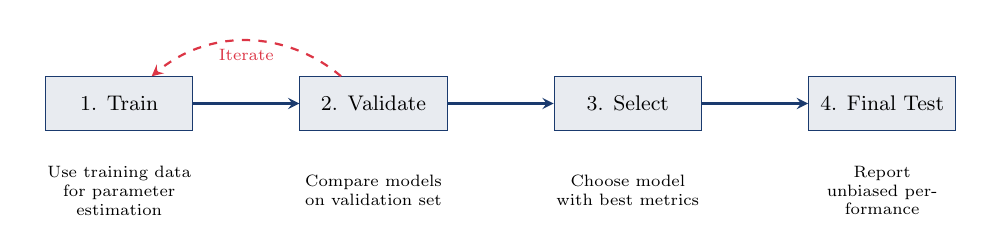
\begin{tikzpicture}[node distance=1.8cm, scale=0.85, transform shape]
        \tikzstyle{process} = [rectangle, minimum width=2.2cm, minimum height=0.8cm, text centered, draw=MainBlue, fill=MainBlue!10, font=\small]
        \tikzstyle{arrow} = [->, >=stealth, thick, MainBlue]

        % Nodes
        \node (train) [process] {1. Train};
        \node (validate) [process, right of=train, xshift=2cm] {2. Validate};
        \node (select) [process, right of=validate, xshift=2cm] {3. Select};
        \node (test) [process, right of=select, xshift=2cm] {4. Final Test};

        % Arrows
        \draw [arrow] (train) -- (validate);
        \draw [arrow] (validate) -- (select);
        \draw [arrow] (select) -- (test);

        % Feedback loop
        \draw [arrow, dashed, Crimson] (validate) to[bend right=40] node[below, font=\scriptsize] {Iterate} (train);

        % Labels below
        \node [below of=train, yshift=0.5cm, font=\scriptsize, text width=2.5cm, align=center] {Use training data\\for parameter\\estimation};
        \node [below of=validate, yshift=0.5cm, font=\scriptsize, text width=2.5cm, align=center] {Compare models\\on validation set};
        \node [below of=select, yshift=0.5cm, font=\scriptsize, text width=2.5cm, align=center] {Choose model\\with best metrics};
        \node [below of=test, yshift=0.5cm, font=\scriptsize, text width=2.5cm, align=center] {Report\\unbiased performance};
    \end{tikzpicture}
    \end{center}

    \vspace{0.15cm}

    \begin{alertblock}{Critical Rule}
        \begin{itemize}\setlength{\itemsep}{0pt}
            \item \textbf{Never use the test set for selection!}
            \begin{itemize}
                \item Use it only for final evaluation
            \end{itemize}
            \item \textbf{Avoid data leakage}
            \begin{itemize}
                \item Overly optimistic performance estimates
            \end{itemize}
        \end{itemize}
    \end{alertblock}
\end{frame}

\begin{frame}{Real Data: Comparing Forecasts}
    \vspace{0.3cm}
    \begin{center}
        \includegraphics[width=0.75\textwidth, height=0.38\textheight, keepaspectratio]{real_data_forecast_comparison.pdf}
    \end{center}
    \vspace{-0.1cm}
    \quantlet{TSA\_ch0\_forecast\_eval}{https://github.com/QuantLet/TSA/tree/main/TSA_ch0/TSA_ch0_forecast_eval}
    \begin{exampleblock}{Interpretation}
        \begin{itemize}\setlength{\itemsep}{0pt}
            \item \textbf{Data}: airline passengers
            \item \textbf{Best}: multiplicative Holt-Winters --- ideal for data with growing seasonality
        \end{itemize}
    \end{exampleblock}
\end{frame}

\begin{frame}{Forecast Performance Across Different Datasets}
    \vspace{0.3cm}
    \begin{center}
        \includegraphics[width=0.75\textwidth, height=0.38\textheight, keepaspectratio]{multiple_series_comparison.pdf}
    \end{center}
    \vspace{-0.1cm}
    \quantlet{TSA\_ch0\_forecast\_eval}{https://github.com/QuantLet/TSA/tree/main/TSA_ch0/TSA_ch0_forecast_eval}
    \begin{exampleblock}{Interpretation}
        \begin{itemize}\setlength{\itemsep}{0pt}
            \item \textbf{Different series}: require different models
            \item \textbf{Seasonal data}: prefer seasonal methods
            \item \textbf{No universal model}: test multiple approaches
        \end{itemize}
    \end{exampleblock}
\end{frame}

%=============================================================================
% SECTION 5: SEASONALITY MODELING
%=============================================================================
\section{Seasonality Modeling}

\begin{frame}{Modeling Seasonality: Two Approaches}
    \vspace{-0.2cm}
    \begin{columns}[T]
        \begin{column}{0.48\textwidth}
            \begin{block}{1. Dummy Variables}
                \begin{itemize}\setlength{\itemsep}{0pt}
                    \item \textbf{Model}: $X_t = \mu + \sum_{j=1}^{s-1}\gamma_j D_{jt} + \varepsilon_t$
                    \item $D_{jt} = 1$ if $t$ in season $j$
                    \item $s-1$ parameters
                    \item Any seasonal pattern
                \end{itemize}
            \end{block}
        \end{column}
        \begin{column}{0.48\textwidth}
            \begin{exampleblock}{2. Fourier Terms}
                \begin{itemize}\setlength{\itemsep}{0pt}
                    \item {\small \textbf{Model}: $X_t = \mu + \sum_{k=1}^{K}\!\left[\alpha_k\sin\!\left(\frac{2\pi k t}{s}\right) + \beta_k\cos\!\left(\frac{2\pi k t}{s}\right)\right]$}
                    \item Sinusoidal functions
                    \item $2K$ parameters
                    \item Smooth patterns
                \end{itemize}
            \end{exampleblock}
        \end{column}
    \end{columns}

    \vspace{0.1cm}

    \begin{alertblock}{Trade-off}
        \begin{itemize}\setlength{\itemsep}{0pt}
            \item \textbf{Dummy variables}
            \begin{itemize}
                \item Any seasonal pattern, but more parameters
            \end{itemize}
            \item \textbf{Fourier terms}
            \begin{itemize}
                \item Smooth patterns, fewer parameters
            \end{itemize}
        \end{itemize}
    \end{alertblock}
\end{frame}

\begin{frame}{Dummy Variables vs Fourier Terms}
    \vspace{0.3cm}
    \begin{center}
        \includegraphics[width=0.75\textwidth, height=0.38\textheight, keepaspectratio]{seasonality_fourier_dummies.pdf}
    \end{center}
    \vspace{-0.1cm}
    \quantlet{TSA\_ch0\_seasonal}{https://github.com/QuantLet/TSA/tree/main/TSA_ch0/TSA_ch0_seasonal}
    \begin{block}{Comparison}
        \begin{itemize}\setlength{\itemsep}{0pt}
            \item \textbf{Dummy variables}: capture any shape, require $s-1$ parameters
            \item \textbf{Fourier terms}: only $2K$ parameters, smooth sinusoidal patterns
        \end{itemize}
    \end{block}
\end{frame}

\begin{frame}{Choosing Between Dummy and Fourier}
    \begin{center}
    \small
    \begin{tabular}{lcc}
        \toprule
        \textbf{Criterion} & \textbf{Dummy} & \textbf{Fourier} \\
        \midrule
        Parameters (monthly) & 11 & $2K$ (often 4--6) \\
        Seasonal pattern & Any shape & Smooth/sinusoidal \\
        Interpretation & Direct (monthly effects) & Frequency components \\
        High-frequency seasons & Many parameters & Efficient \\
        Multiple seasonality & Complex & Easy (add terms) \\
        \bottomrule
    \end{tabular}
    \end{center}

    \vspace{0.1cm}

    \begin{exampleblock}{Recommendations}
        \begin{itemize}\setlength{\itemsep}{0pt}
            \item \textbf{Use Dummy}
            \begin{itemize}
                \item Irregular patterns, interpretable coefficients
            \end{itemize}
            \item \textbf{Use Fourier}
            \begin{itemize}
                \item Smooth patterns, high-frequency seasonality
                \item Used in TBATS and Prophet
            \end{itemize}
        \end{itemize}
    \end{exampleblock}
\end{frame}

%=============================================================================
% SECTION 6: HANDLING TREND AND SEASONALITY
%=============================================================================
\section{Handling Trend and Seasonality}

\begin{frame}{Why Do We Remove Trend and Seasonality?}
    \vspace{-0.2cm}
    \begin{columns}[T]
        \begin{column}{0.48\textwidth}
            \begin{block}{Reasons for Detrending}
                \begin{itemize}\setlength{\itemsep}{0pt}
                    \item Stationarity requirement
                    \item Focus on fluctuations
                    \item Avoiding spurious regression
                    \item Enabling valid inference
                \end{itemize}
            \end{block}
        \end{column}
        \begin{column}{0.48\textwidth}
            \begin{exampleblock}{Reasons for Deseasonalizing}
                \begin{itemize}\setlength{\itemsep}{0pt}
                    \item Revealing the underlying trend
                    \item Cross-season comparisons
                    \item Simplifying modeling
                    \item Focus on the irregular component
                \end{itemize}
            \end{exampleblock}
        \end{column}
    \end{columns}

    \vspace{0.1cm}

    \begin{alertblock}{Important}
        \begin{itemize}\setlength{\itemsep}{0pt}
            \item \textbf{We model the transformed series}
            \begin{itemize}
                \item With trend and seasonality removed
            \end{itemize}
            \item \textbf{We reverse the transformation}
            \begin{itemize}
                \item Bring the forecast back to the original scale
            \end{itemize}
        \end{itemize}
    \end{alertblock}
\end{frame}

\begin{frame}{Detrending Methods}
    \begin{columns}[T]
        \column{0.55\textwidth}
        \begin{block}{Six Common Detrending Approaches}
            \begin{itemize}\setlength{\itemsep}{0pt}
                \item \textbf{Differencing}: $\Delta X_t = X_t - X_{t-1}$
                \begin{itemize}
                    \item Most commonly used, removes stochastic trend
                \end{itemize}
                \item \textbf{Linear regression}: $\hat{T}_t = \hat{\beta}_0 + \hat{\beta}_1 t$
                \item \textbf{Polynomial}: higher-order polynomial
                \item \textbf{HP filter}: balance between fit and smoothness
                \item \textbf{Moving average}: $\hat{T}_t = MA_q(X_t)$
                \item \textbf{LOESS}: local polynomial regression
            \end{itemize}
        \end{block}
        \column{0.43\textwidth}
        \begin{exampleblock}{The Choice Depends on}
            \begin{itemize}\setlength{\itemsep}{0pt}
                \item \textbf{Nature of the trend}
                \begin{itemize}
                    \item Deterministic vs stochastic
                \end{itemize}
                \item \textbf{Purpose of the analysis}
                \begin{itemize}
                    \item Forecasting vs descriptive analysis
                \end{itemize}
            \end{itemize}
        \end{exampleblock}
    \end{columns}
\end{frame}

\begin{frame}{Detrending Methods: Comparison}
    \vspace{0.3cm}
    \begin{center}
        \includegraphics[width=0.75\textwidth, height=0.38\textheight, keepaspectratio]{detrending_methods.pdf}
    \end{center}
    \vspace{-0.1cm}
    \quantlet{TSA\_ch0\_detrending}{https://github.com/QuantLet/TSA/tree/main/TSA_ch0/TSA_ch0_detrending}
    \begin{alertblock}{Key Idea}
        \begin{itemize}\setlength{\itemsep}{0pt}
            \item \textbf{Different methods}: produce different residuals
            \item \textbf{Choose by trend type}: consider the analysis objectives
        \end{itemize}
    \end{alertblock}
\end{frame}

\begin{frame}{Trend Estimation: Multiple Approaches}
    \vspace{0.3cm}
    \begin{center}
        \includegraphics[width=0.75\textwidth, height=0.38\textheight, keepaspectratio]{trend_estimation_comparison.pdf}
    \end{center}
    \vspace{-0.1cm}
    \quantlet{TSA\_ch0\_detrending}{https://github.com/QuantLet/TSA/tree/main/TSA_ch0/TSA_ch0_detrending}
    \begin{exampleblock}{Method Comparison}
        \begin{itemize}\setlength{\itemsep}{0pt}
            \item \textbf{Moving average}: simple but with lag
            \item \textbf{Polynomial regression}: flexible, parametric
            \item \textbf{HP filter}: macroeconomic standard
        \end{itemize}
    \end{exampleblock}
\end{frame}

\begin{frame}{The Hodrick-Prescott (HP) Filter}
    \begin{defn}[HP Filter]
        \begin{itemize}\setlength{\itemsep}{0pt}
            \item \textbf{HP filter}: decomposes $X_t$ into trend $\tau_t$ and cycle $c_t$: $X_t = \tau_t + c_t$
            \vspace{-0.2cm}
            {\small\[
                \min_{\{\tau_t\}} \left\{ \sum_{t=1}^{T}(X_t - \tau_t)^2 + \lambda \sum_{t=2}^{T-1}[(\tau_{t+1} - \tau_t) - (\tau_t - \tau_{t-1})]^2 \right\}
            \]}
            \vspace{-0.3cm}
        \end{itemize}
    \end{defn}

    \begin{columns}[T]
        \column{0.48\textwidth}
        \begin{block}{Interpretation}
            \begin{itemize}\setlength{\itemsep}{0pt}
                \item \textbf{First term}
                \begin{itemize}
                    \item Goodness of fit
                \end{itemize}
                \item \textbf{Second term}
                \begin{itemize}
                    \item Smoothness penalty
                \end{itemize}
                \item \textbf{$\lambda$}
                \begin{itemize}
                    \item Controls the balance between fidelity and smoothness
                \end{itemize}
            \end{itemize}
        \end{block}
        \column{0.5\textwidth}
        \begin{exampleblock}{Standard $\lambda$ Values (Ravn-Uhlig)}
            \begin{itemize}\setlength{\itemsep}{0pt}
                \item \textbf{Annual}
                \begin{itemize}
                    \item $\lambda = 6.25$
                \end{itemize}
                \item \textbf{Quarterly}
                \begin{itemize}
                    \item $\lambda = 1600$ (macroeconomic standard)
                \end{itemize}
                \item \textbf{Monthly}
                \begin{itemize}
                    \item $\lambda = 129600$
                \end{itemize}
            \end{itemize}
        \end{exampleblock}
    \end{columns}
\end{frame}

\begin{frame}{HP Filter: Effect of $\lambda$}
    \vspace{0.3cm}
    \begin{center}
        \includegraphics[width=0.75\textwidth, height=0.38\textheight, keepaspectratio]{ch1_hp_filter_lambda.png}
    \end{center}
    \vspace{-0.1cm}
    \quantlet{TSA\_ch0\_detrending}{https://github.com/QuantLet/TSA/tree/main/TSA_ch0/TSA_ch0_detrending}
    \begin{block}{Trade-off}
        \begin{itemize}\setlength{\itemsep}{0pt}
            \item \textbf{Small $\lambda$}: flexible trend, follows the data closely
            \item \textbf{Large $\lambda$}: smooth trend, approaches a linear trend
        \end{itemize}
    \end{block}
\end{frame}

\begin{frame}{HP Filter: Business Cycle Extraction}
    \vspace{0.3cm}
    \begin{center}
        \includegraphics[width=0.75\textwidth, height=0.38\textheight, keepaspectratio]{ch1_hp_filter_cycle.png}
    \end{center}
    \vspace{-0.1cm}
    \quantlet{TSA\_ch0\_detrending}{https://github.com/QuantLet/TSA/tree/main/TSA_ch0/TSA_ch0_detrending}
    \begin{exampleblock}{Application}
        \begin{itemize}\setlength{\itemsep}{0pt}
            \item \textbf{Macroeconomics}: business cycle extraction
            \item \textbf{Common series}: GDP, unemployment, inflation
        \end{itemize}
    \end{exampleblock}
\end{frame}

\begin{frame}{HP Filter: Limitations}
    \begin{columns}[T]
        \column{0.48\textwidth}
        \begin{alertblock}{Known Issues}
            \begin{itemize}\setlength{\itemsep}{0pt}
                \item \textbf{Endpoint instability}
                \begin{itemize}
                    \item Trend estimates unreliable at the beginning and end
                \end{itemize}
                \item \textbf{Spurious cycles}
                \begin{itemize}
                    \item Can create artificial dynamics
                \end{itemize}
                \item \textbf{Choice of $\lambda$}
                \begin{itemize}
                    \item Results sensitive to the parameter
                \end{itemize}
            \end{itemize}
        \end{alertblock}
        \column{0.5\textwidth}
        \begin{exampleblock}{Alternatives}
            \begin{itemize}\setlength{\itemsep}{0pt}
                \item \textbf{Band-pass filters}: Baxter-King, Christiano-Fitzgerald
                \begin{itemize}
                    \item Isolate specific frequencies
                \end{itemize}
                \item \textbf{Hamilton filter}: regression-based
                \item \textbf{Unobserved components}: state-space models
            \end{itemize}
        \end{exampleblock}
    \end{columns}

    \vspace{0.1cm}

    \begin{block}{Hamilton's Critique (2018)}
        \begin{itemize}\setlength{\itemsep}{0pt}
            \item ``Why You Should Never Use the Hodrick-Prescott Filter''
            \begin{itemize}
                \item Suggests using regression on lagged values
            \end{itemize}
        \end{itemize}
    \end{block}
\end{frame}

\begin{frame}{Seasonal Adjustment Methods}
    \begin{block}{Four Approaches for Seasonal Adjustment}
        \begin{itemize}\setlength{\itemsep}{0pt}
            \item \textbf{Seasonal differencing}: $\Delta_s X_t = X_t - X_{t-s}$
            \begin{itemize}
                \item Removes periodic pattern, simple to apply
            \end{itemize}
            \item \textbf{Division} (multiplicative): $X_t^{adj} = X_t / \hat{S}_t$
            \item \textbf{Subtraction} (additive): $X_t^{adj} = X_t - \hat{S}_t$
            \item \textbf{X-13ARIMA-SEATS}: official US Census Bureau standard
            \begin{itemize}
                \item Sophisticated method, used by statistical institutes
            \end{itemize}
        \end{itemize}
    \end{block}

    \vspace{0.1cm}

    \begin{exampleblock}{Seasonal Period $s$}
        \begin{itemize}\setlength{\itemsep}{0pt}
            \item Monthly: $s=12$ \quad|\quad Quarterly: $s=4$
        \end{itemize}
    \end{exampleblock}
\end{frame}

\begin{frame}{Seasonal Adjustment: Visualization}
    \vspace{0.3cm}
    \begin{center}
        \includegraphics[width=0.75\textwidth, height=0.38\textheight, keepaspectratio]{seasonal_adjustment.pdf}
    \end{center}
    \vspace{-0.1cm}
    \quantlet{TSA\_ch0\_seasonal}{https://github.com/QuantLet/TSA/tree/main/TSA_ch0/TSA_ch0_seasonal}
    \begin{block}{Result}
        \begin{itemize}\setlength{\itemsep}{0pt}
            \item \textbf{Seasonally adjusted series}: reveals the underlying trend, removes periodic fluctuations
        \end{itemize}
    \end{block}
\end{frame}

\begin{frame}{Deterministic vs Stochastic Trend}
    \vspace{-0.2cm}
    \begin{columns}[T]
        \begin{column}{0.48\textwidth}
            \begin{block}{Deterministic Trend}
                \begin{itemize}\setlength{\itemsep}{0pt}
                    \item \textbf{Model}: $X_t = \beta_0 + \beta_1 t + \varepsilon_t$
                    \item \textbf{Characteristics}:
                    \begin{itemize}
                        \item Trend is a function of time
                        \item $\varepsilon_t$ is stationary
                    \end{itemize}
                    \item \textbf{Method}: detrend by regression
                \end{itemize}
            \end{block}
        \end{column}
        \begin{column}{0.48\textwidth}
            \begin{exampleblock}{Stochastic Trend}
                \begin{itemize}\setlength{\itemsep}{0pt}
                    \item \textbf{Model}: $X_t = X_{t-1} + \varepsilon_t$
                    \item \textbf{Characteristics}:
                    \begin{itemize}
                        \item Random walk component
                        \item $\Delta X_t$ is stationary
                    \end{itemize}
                    \item \textbf{Method}: detrend by differencing
                \end{itemize}
            \end{exampleblock}
        \end{column}
    \end{columns}

    \vspace{0.1cm}

    \begin{alertblock}{Wrong Method = Problems}
        \begin{itemize}\setlength{\itemsep}{0pt}
            \item \textbf{Differencing a deterministic trend} $\rightarrow$ over-differencing
            \begin{itemize}
                \item Introduces artificial dependence in the series
            \end{itemize}
            \item \textbf{Regression on a stochastic trend} $\rightarrow$ spurious regression
            \begin{itemize}
                \item Invalid statistical results
            \end{itemize}
        \end{itemize}
    \end{alertblock}
\end{frame}

\begin{frame}{Example: Deterministic Trend}
    \vspace{0.3cm}
    \begin{center}
        \includegraphics[width=0.75\textwidth, height=0.38\textheight, keepaspectratio]{deterministic_trend_example.pdf}
    \end{center}
    \vspace{-0.1cm}
    \quantlet{TSA\_ch0\_detrending}{https://github.com/QuantLet/TSA/tree/main/TSA_ch0/TSA_ch0_detrending}
    \begin{exampleblock}{Key}
        \begin{itemize}\setlength{\itemsep}{0pt}
            \item \textbf{Method}: \textcolor{Crimson}{regression}
            \item \textbf{Result}: stationary residuals, ACF decays rapidly
        \end{itemize}
    \end{exampleblock}
\end{frame}

\begin{frame}{Example: Stochastic Trend (Random Walk)}
    \vspace{0.3cm}
    \begin{center}
        \includegraphics[width=0.75\textwidth, height=0.38\textheight, keepaspectratio]{stochastic_trend_example.pdf}
    \end{center}
    \vspace{-0.1cm}
    \quantlet{TSA\_ch0\_detrending}{https://github.com/QuantLet/TSA/tree/main/TSA_ch0/TSA_ch0_detrending}
    \begin{exampleblock}{Key}
        \begin{itemize}\setlength{\itemsep}{0pt}
            \item \textbf{Method}: \textcolor{Crimson}{differencing}
            \item \textbf{Result}: differences are stationary (white noise)
        \end{itemize}
    \end{exampleblock}
\end{frame}

\begin{frame}{Side-by-Side Comparison}
    \vspace{0.3cm}
    \begin{center}
        \includegraphics[width=0.75\textwidth, height=0.38\textheight, keepaspectratio]{trend_comparison_sidebyside.pdf}
    \end{center}
    \vspace{-0.1cm}
    \quantlet{TSA\_ch0\_detrending}{https://github.com/QuantLet/TSA/tree/main/TSA_ch0/TSA_ch0_detrending}
    \begin{alertblock}{Remember}
        \begin{itemize}\setlength{\itemsep}{0pt}
            \item \textbf{Deterministic trend}: use regression --- trend is a predictable function of time
            \item \textbf{Stochastic trend}: use differencing --- trend contains a random component
        \end{itemize}
    \end{alertblock}
\end{frame}

%=============================================================================
\section{AI Use Case}
%=============================================================================

\begin{frame}{AI Exercise: Critical Thinking}
    \vspace{-3mm}
    \begin{block}{\footnotesize Prompt to test in ChatGPT / Claude / Copilot}
        {\footnotesize
        ``Using yfinance, download AAPL stock data. I want to see what patterns exist and predict where the price will go next year. Make it look professional with charts.''
        }
    \end{block}
    \vspace{-2mm}
    {\footnotesize
    \textbf{Exercise}:
    \begin{enumerate}\setlength{\itemsep}{0pt}
        \item Run the prompt in an LLM of your choice and critically analyze the response.
        \item What type of decomposition does the model choose? Is it correct? Justify.
        \item How does it evaluate forecast quality? Is the metric computed correctly?
        \item Check the residuals --- do they show unexplained structure?
        \item Rewrite the analysis correctly and compare with a seasonal na\"ive benchmark.
    \end{enumerate}
    }
    \vspace{-2mm}
    \begin{alertblock}{}
        {\footnotesize \textbf{Warning}: AI-generated code may run without errors and look professional. \textit{That does not mean it is correct.}}
    \end{alertblock}
\end{frame}

%=============================================================================
\section{Summary}
%=============================================================================

\begin{frame}{Summary}
    \begin{block}{What We Learned in This Chapter}
        \begin{itemize}\setlength{\itemsep}{1pt}
            \item Time Series Definition and Characteristics
            \begin{itemize}
                \item Sequence of temporally ordered observations with dependence
            \end{itemize}
            \item Decomposition (Additive vs Multiplicative)
            \begin{itemize}
                \item Components: Trend-Cycle + Seasonal + Residual
            \end{itemize}
            \item Exponential Smoothing Methods
            \begin{itemize}
                \item SES (level), Holt (+ trend), Holt-Winters (+ seasonality), ETS
            \end{itemize}
            \item Forecast Evaluation and Validation
            \begin{itemize}
                \item Metrics: MAE, RMSE, MAPE; Cross-Validation with rolling origin
            \end{itemize}
        \end{itemize}
    \end{block}
    \begin{exampleblock}{Key Idea}
        \begin{itemize}\setlength{\itemsep}{0pt}
            \item \textbf{Understand Before Modeling}:
            \begin{itemize}
                \item Visualize and decompose the data first
                \item Choose additive vs multiplicative based on variance behavior
            \end{itemize}
        \end{itemize}
    \end{exampleblock}
\end{frame}

\begin{frame}{Quick Quiz}
    \begin{block}{Test Your Knowledge}
        \begin{itemize}\setlength{\itemsep}{4pt}
            \item[\textcolor{MainBlue}{\textbf{1.}}] What is the difference between additive and multiplicative decomposition?
            \item[\textcolor{MainBlue}{\textbf{2.}}] When should you use Holt-Winters instead of SES?
            \item[\textcolor{MainBlue}{\textbf{3.}}] Why can't we use standard k-fold CV for time series?
            \item[\textcolor{MainBlue}{\textbf{4.}}] What does $\alpha = 0.9$ mean in exponential smoothing?
            \item[\textcolor{MainBlue}{\textbf{5.}}] How do you distinguish between a deterministic and stochastic trend?
        \end{itemize}
    \end{block}
\end{frame}

\begin{frame}{Quiz Answers}
    {\footnotesize
    \begin{exampleblock}{Answers}
        \begin{itemize}\setlength{\itemsep}{1pt}
            \item[\textcolor{MainBlue}{\textbf{1.}}] \textbf{Additive vs multiplicative}: additive when seasonal amplitude is constant; multiplicative when it grows with the level
            \item[\textcolor{MainBlue}{\textbf{2.}}] \textbf{Holt-Winters}: when data have trend AND seasonality; SES handles only the level
            \item[\textcolor{MainBlue}{\textbf{3.}}] \textbf{CV}: standard k-fold ignores temporal order $\rightarrow$ data leakage
            \item[\textcolor{MainBlue}{\textbf{4.}}] \textbf{$\alpha = 0.9$}: high weight on recent observations, reacts quickly but more volatile
            \item[\textcolor{MainBlue}{\textbf{5.}}] \textbf{Trend}: deterministic $\rightarrow$ function of time (regression); stochastic $\rightarrow$ random walk (differencing)
        \end{itemize}
    \end{exampleblock}
    }
\end{frame}

\begin{frame}{What's Next?}
    \begin{center}
    \begin{minipage}{0.85\textwidth}
    \begin{block}{Chapter 1: Stochastic Processes and Stationarity}
        \begin{itemize}\setlength{\itemsep}{0pt}
            \item \textbf{Stochastic Processes}: mathematical foundation, random variables indexed by time
            \item \textbf{Stationarity}: strict (invariant distribution) vs weak (invariant moments)
            \item \textbf{Fundamental Processes}: white noise and random walk $\rightarrow$ building blocks for ARIMA
            \item \textbf{ACF and PACF}: tools for model identification
        \end{itemize}
    \end{block}
    \end{minipage}
    \end{center}

    \vspace{0.3cm}
    \begin{center}
        \Large\textcolor{MainBlue}{Questions?}
    \end{center}
\end{frame}

%=============================================================================
% BIBLIOGRAPHY
%=============================================================================
\begin{frame}{Bibliography I}
    \begin{block}{Time Series Fundamentals}
        {\small
        \begin{itemize}\setlength{\itemsep}{0pt}
            \item Wold, H. (1938). \textit{A Study in the Analysis of Stationary Time Series}, Almqvist \& Wiksell.
            \item Hamilton, J.D. (1994). \textit{Time Series Analysis}, Princeton University Press.
            \item Brockwell, P.J., \& Davis, R.A. (2016). \textit{Introduction to Time Series and Forecasting}, 3rd ed., Springer.
        \end{itemize}
        }
    \end{block}

    \begin{exampleblock}{Decomposition and Exploratory Analysis}
        {\small
        \begin{itemize}\setlength{\itemsep}{0pt}
            \item Cleveland, R.B., Cleveland, W.S., McRae, J.E., \& Terpenning, I. (1990). STL: A Seasonal-Trend Decomposition Procedure Based on Loess, \textit{Journal of Official Statistics}, 6(1), 3--33.
            \item Hyndman, R.J., \& Athanasopoulos, G. (2021). \textit{Forecasting: Principles and Practice}, 3rd ed., OTexts.
        \end{itemize}
        }
    \end{exampleblock}
\end{frame}

\begin{frame}{Bibliography II}
    \begin{block}{Exponential Smoothing and ETS Fundamentals}
        {\small
        \begin{itemize}\setlength{\itemsep}{0pt}
            \item Holt, C.C. (1957/2004). Forecasting Seasonals and Trends by Exponentially Weighted Moving Averages, \textit{International Journal of Forecasting}, 20(1), 5--10.
            \item Winters, P.R. (1960). Forecasting Sales by Exponentially Weighted Moving Averages, \textit{Management Science}, 6(3), 324--342.
            \item Hyndman, R.J., Koehler, A.B., Ord, J.K., \& Snyder, R.D. (2008). \textit{Forecasting with Exponential Smoothing: The State Space Approach}, Springer.
        \end{itemize}
        }
    \end{block}

    \begin{exampleblock}{Online Resources and Code}
        {\small
        \begin{itemize}\setlength{\itemsep}{0pt}
            \item \textbf{Quantlet}: \url{https://quantlet.com} $\rightarrow$ Code repository for statistics
            \item \textbf{Quantinar}: \url{https://quantinar.com} $\rightarrow$ Learning platform for quantitative methods
            \item \textbf{GitHub TSA\_ch0}: \url{https://github.com/QuantLet/TSA/tree/main/TSA_ch0}
        \end{itemize}
        }
    \end{exampleblock}
\end{frame}

\end{document}
